\chapter{実装}
\label{make}
本章では実装したヘルメットのハードウェアとソフトウェアを説明する.

\section{ハードウェア}
提案手法に用いる圧力センサを搭載したヘルメットを実装した.デバイスの構成を図\ref{device},プロトタイプデバイスの写真を図\ref{met_over}に示す.

圧力値を正しく取得するには,センサとヘルメット装着者の頭部が密着している必要があるため,フルフェイス型ヘルメット(B\&B社製BB100)を用いた.圧力センサとしてインターリンクエレクトロニクス社製のFSR402およびFSR402 ShortTailを合計32個使用した.
マイコンとしてArduino MEGA2560 R3を使用した.

実装したプロトタイプデバイスの内部を図\ref{met_in}に示す.今回用いたヘルメットはフリーサイズであり,また内装の脱着が困難であったため,頭頂部の内装を取り外して,新たに厚みのあるウレタンスポンジを取り付けた.図\ref{sensor}のようにウレタンスポンジの中央部に切り込みを入れて圧力センサを挿し込んだ.圧力センサは頭頂部に4個,頭頂部周囲に16個,後頭部に6個,左右チークパッド部に6個の合計32個を搭載した.配線はヘルメットの頭頂部にドリルで開けた穴から,ヘルメット外部に取り付けた10KΩの抵抗を配線してあるプリント基板を経由して,Arduino MEGA2560 R3の5V電源,GND,アナログ入力ポートに接続した.このプリント基板を図\ref{print}に示す.プリント基板は取り外しが可能なように,ヘルメットのシールド固定用に開けられたネジ穴を用いて左頬部分にボルトで固定している.

\begin{figure}[!t]
  \begin{center}
    \includegraphics[width=0.65\linewidth]{figure/device.eps}
  \end{center}
  \caption{デバイス構成}
  \label{device}
\end{figure}

\begin{figure}[!t]
  \begin{center}
    \includegraphics[width=0.6\linewidth]{figure/met_over.eps}
  \end{center}
  \caption{プロトタイプデバイスの全体図}
  \label{met_over}
\end{figure}

\begin{figure}[!t]
  \begin{center}
    \includegraphics[width=0.6\linewidth]{figure/met_in.eps}
  \end{center}
  \caption{プロトタイプデバイスの内部}
  \label{met_in}
\end{figure}

\begin{figure}[!t]
  \begin{center}
    \includegraphics[width=0.6\linewidth]{figure/sensor.eps}
  \end{center}
  \caption{センサの実装方法}
  \label{sensor}
\end{figure}

\begin{figure}[!t]
  \begin{center}
    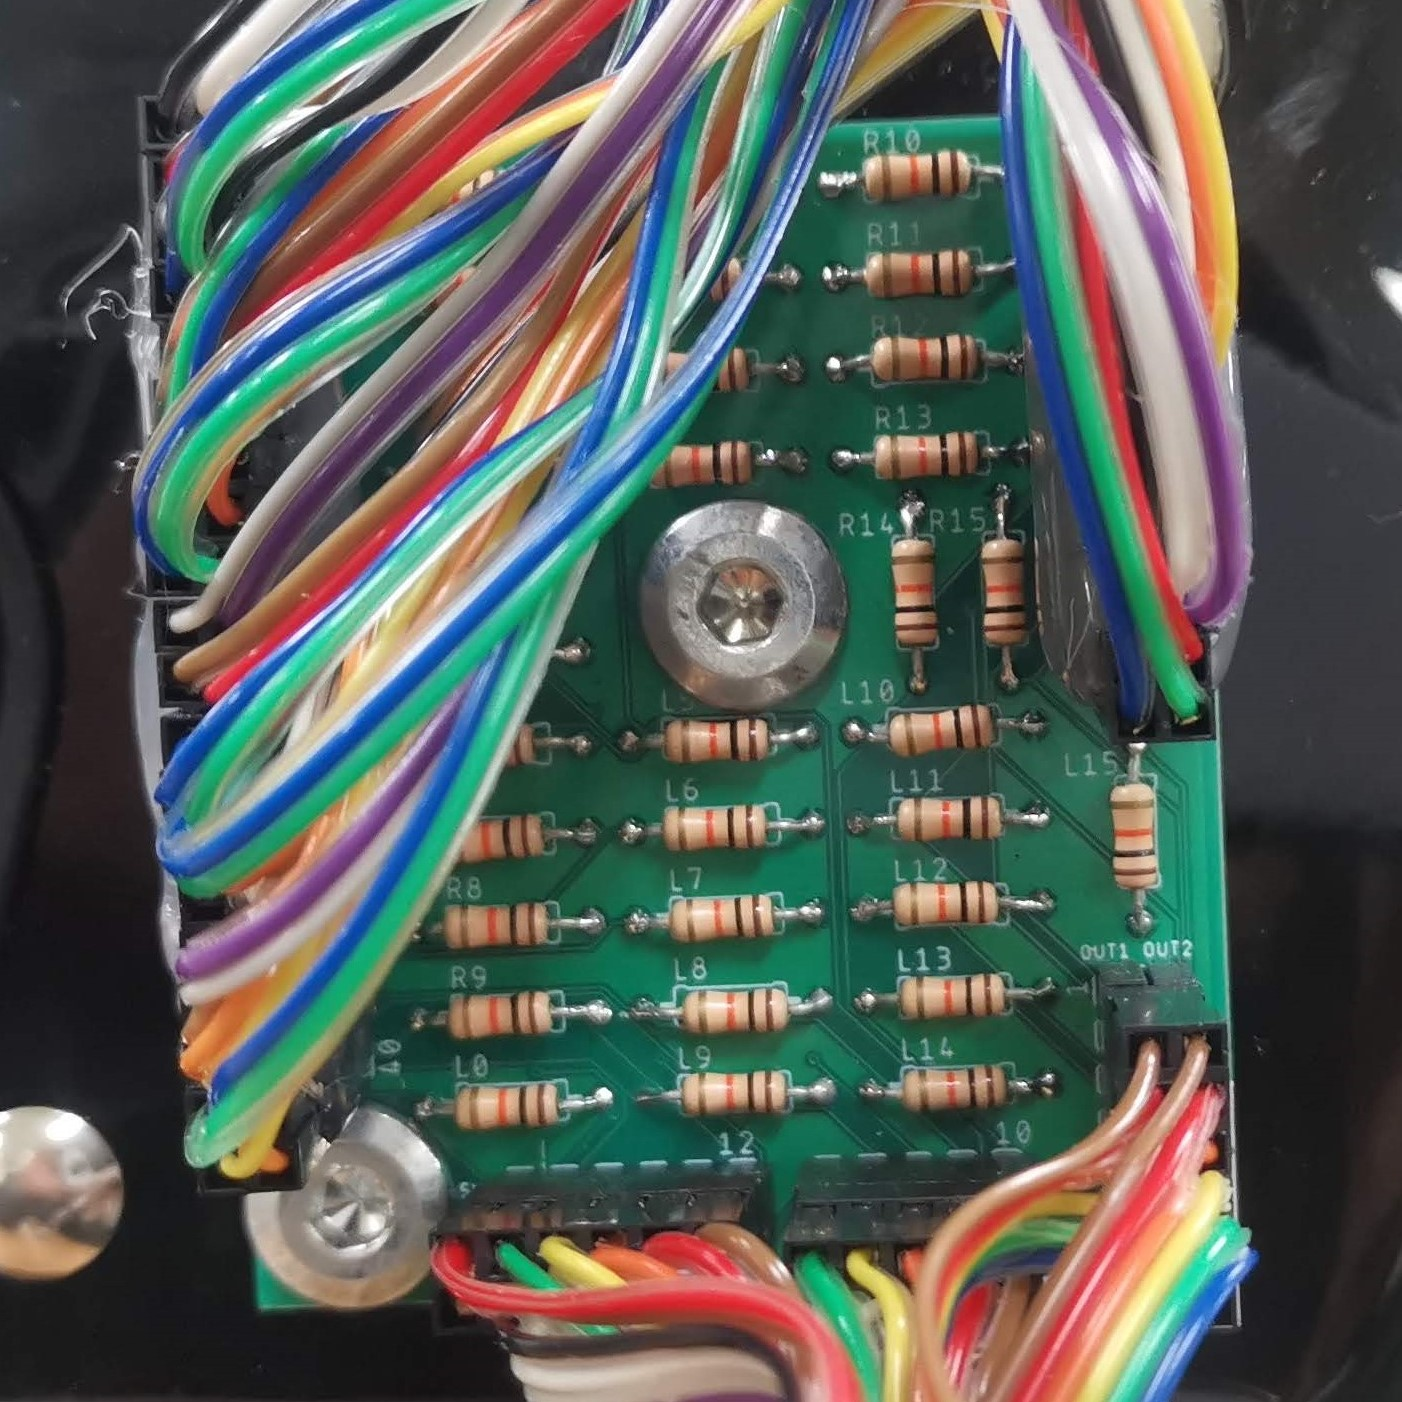
\includegraphics[width=0.6\linewidth]{figure/print.eps}
  \end{center}
  \caption{プリント基板}
  \label{print}
\end{figure}

\section{ソフトウェア}
Arduino MEGAのプログラムはArduinoIDEで実装した.マイコンからコンピュータへのデータの受信はPythonで実装し,センサデータをコンピュータ上にcsv形式で保存する.
データの解析はPythonで実装し,事前に収集したセンサデータのcsvファイルを読み出し,sklearn.covariance.MinCovDetを用いて分散共分散行列を計算する.その分散共分散行列の逆行列から,scipy.spatial.distanceを用いて学習データ$\bm{x}_i$のすべてに対する入力データ$\bm{y}$のマハラノビス距離を計算する.
sklearn.covariance.MinCovDetとは,異常値に対して頑健な分散共分散行列の推定アルゴリズムであるMinimum Covariance Determinant (MCD)を高速化したFast-MCD\cite{fast_mcd}を実装したscikit-learnのライブラリである.また,scipy.spatial.distanceとは,様々な距離計算の関数を実装したSciPyのライブラリである.